\documentclass[11pt]{article}
\usepackage[utf8]{inputenc}
\usepackage[T1]{fontenc}
\usepackage{amsmath}
\usepackage{amsfonts}
\usepackage{amssymb}
\usepackage[version=4]{mhchem}
\usepackage{stmaryrd}
\usepackage{graphicx}
\usepackage[export]{adjustbox}
\graphicspath{ {./images/} }

\begin{document}
Fixed-Income Arbitrage

Fixed-income arbitrage involves simultaneous long and short positions in fixed-income securities with the expectation that over the investment holding period, the security prices will converge toward a similar valuation standard.

\section*{The Core of Fixed-Income Arbitrage Strategies}
At the core of any arbitrage strategy is a model of how prices should behave. This model may be based on theory, empirical observations, or both. The arbitrage is often performed on a pair of securities with a long position in one security offset by a short position in the other security. However, the arbitrage can involve any number of longs and shorts.

An example of a three-security trade is as follows: Assume that based on theoretical reasons or past observations, a fund manager predicts that the yield on 9-month debt will trade at a particular relationship to the yields on 6-month and 12-month debt. Assume that the fund manager predicts that the 9-month yield will trade within five basis points of the mean between the other two yields in a particular market. The fund manager might take a long position in the 9-month debt whenever its yield trades above this relationship, while taking offsetting short positions in the 6-month and 12-month bonds. The fund manager is speculating that the yield on the 9-month debt will decline relative to the average yields of the other two bonds as its yield returns toward the long-term relationship that the fund manager predicts. Note that the manager is not speculating necessarily that the 9-month yield is absolutely high or that the 6-and 12-month yields are absolutely low. Rather, the manager is speculating on the relative values and, in particular, that the relative values will converge as predicted by the manager's model.

Fixed-income arbitrage managers search continuously for pricing inefficiencies across all fixed-income markets. These arbitrage strategies are similar to the traditional goal of buying low and selling high. However, in arbitrage, the trade is based on relative value rather than absolute value, and the goal is to hedge the aggregated position against all risks other than the specific behavior on which the manager is speculating. The arbitrageur hedges the positions against market factors such as credit risks and general interest rate risks, then waits for the relatively undervalued security (or securities) to increase in value, the relatively overvalued security (or securities) to decline in value, or both to occur.

In most cases, trades are designed to be duration-neutral. Duration is a measure of the sensitivity of a fixed-income security to a change in the general level of interest rates, as discussed in Session 2.5, Financial Economics Foundations. A duration-neutral position means that the returns to the position are relatively insensitive to changes in the general level of market interest rates. However, fixed-income positions can also be exposed to other risks, such as changes in credit spreads, changes in yield curve shapes, changes in volatility, and changes in liquidity. Generally, the perceived relative mispricing between fixed-income securities is small. Thus, the potential profit of the fixed-income arbitrageur is typically small relative to the sizes of the long and short positions. By controlling for other risks, the hedge fund manager attempts to generate returns driven solely by the behavior of the pricing discrepancy. If the pricing discrepancy converges over time, the strategy should generate a profit. If the pricing discrepancy diverges further, the positions generate losses.

Given the relatively small potential profits as a proportion of position sizes, hedge fund managers typically add more profit potential through leveraging their portfolios with direct borrowings from their prime brokers or with swaps and other derivative securities. This leverage can lead to substantial positive returns when prices return to their predicted levels, which typically happens in normal markets but can create disastrous losses in turbulent environments. Key issues in such arbitrage strategies are managing liquidity and adjusting the size of the positions as perceived price discrepancies diverge further and further in turbulent markets. If positions are reduced, the fund may have reduced its profit potential when the prospects for future profits are at their highest. However, if positions are maintained or increased as losses mount, the firm runs the risk of being forced to liquidate when price discrepancies and losses are at their highest levels.

\section*{Types of Fixed-Income Arbitrage Strategies}
There are numerous ways to categorize fixed-income arbitrage strategies. Within a particular bond market, positions may be established by anticipating various changes in relationships. These strategies include speculations that the yield curve will become less steeply sloped (yield flattener), that the yield curve will become more steeply sloped (yield steepener), or that portions of the curve will become more curved or less curved (yield butterflies). These are examples of intracurve arbitrage positions because they are based on hedged positions within the same yield curve.

A yield curve is the relationship between the yields of various securities, usually depicted on the vertical axis, and the term to maturity, usually depicted on the horizontal axis. The terms yield curve and term structure of interest rates are often used interchangeably. Sometimes the term structure of interest rates is distinguished from the yield curve because the yield curve plots yields to maturity of coupon bonds, whereas the term structure of interest rates plots actual or hypothetical yields of zero-coupon bonds.

There are also intercurve arbitrage positions, which means arbitrage (hedged positions) using securities related to different yield curves. Examples include swap spread trading (arbitraging differences in swap rates) and carry trades. Carry trades attempt to earn profits from carrying or maintaining long positions in higheryielding assets and short positions in lower-yielding assets without suffering from adverse price movements. For further examples, see Duarte, Longstaff, and Yu. ${ }^{1}$ Jefferson Duarte, Francis A. Longstaff, and Fan Yu (2006), Risk and Return in Fixed-Income Arbitrage: Nickels in Front of a Steamroller? Review of Financial Studies 20 (no. 3): 769-811. They discuss swap-spread arbitrage, yield-curve arbitrage, mortgage arbitrage, volatility arbitrage, and capital-structure arbitrage.

Fixed-income arbitrage funds are often differentiated by the markets in which they speculate. These markets fall into a number of categories, including sovereign debt and asset-backed or mortgage-backed securities.

\section*{Fixed-Income Arbitrage Strategies: Sovereign Debt}
Sovereign debt is debt issued by national governments. Sovereign debt possesses distinct credit risks from corporate debt because governments can choose to default on their obligations even when they are technically able to meet them. Further, most national governments can use monetary policy to alter the value of their currency and thereby change the real value of their outstanding obligations. In other words, most national governments can literally print money to pay their debts but can choose to default anyway. Sovereign debt ranges in creditworthiness from the low-credit-risk obligations of the largest and most secure nations to the obligations of the least creditworthy nations. Fixed-income arbitrage and hedging using the obligations of the US government are illustrated here. Fixed-income arbitrage does not need to use exotic securities. For example, it can be nothing more than buying and selling US Treasury securities. In the US bond market, the most\\
liquid securities are on-the-run US Treasury bonds. On-the-run Treasury bonds are the most currently issued bonds for each common maturity issued by the US Treasury Department (e.g., 3-month, 6-month, and 12-month Treasury bills; 10-year notes; and so forth). There are other US Treasury bonds outstanding (known as off-the-run) that have similar maturities and coupons to the on-the-run Treasury bonds. However, off-the-run bonds were issued much earlier than on-the-run bonds and are now less liquid, as dealers are less actively trading them and many of them have been bought and held by long-term investors. As a result, price discrepancies occur among off-the-run issues, as well as between on-the-run and off-the-run issues. The difference in prices may be very small, just a few 32nds of $1 \%$, but can increase in times of high uncertainty, when there are high and erratic levels of trading as investors shift money into and out of the most liquid US Treasury bonds in response to the market crisis.

Another form of fixed-income arbitrage involves trading among maturity ranges of fixed-income securities, especially those that are relatively close to maturity. This is a form of yield-curve arbitrage. These types of trades are driven by temporary imbalances in the supply of and demand for the securities that apparently cause temporary distortions in the yield curve. Kinks in the yield curve can happen at any maturity and usually reflect a change in liquidity demand around the focal point. These kinks provide an opportunity to speculate on changes in the shape of the yield curve by purchasing and selling Treasury securities that are similar in maturity. Investors who hold bonds can view their returns as being driven not just by shifts in the yield curve but also by the change in a bond's yield if the yield curve remains constant and the maturity of the bond shortens. The process of holding a bond as its yield moves up or down the yield curve due to the passage of time is known as riding the yield curve. Consider a yield curve with an upward slope between the two-year and five-year maturities. The holder of the five-year Treasury bond can profit by rolling down or riding down the yield curve toward the two-year rate if the yield curve does not shift. Rolling down the yield curve is the process of experiencing decreasing yields to maturity as an asset's maturity declines through time in an upward-sloping yield curve environment. In other words, if the yield curve remains static, the five-year Treasury note ages into a lower-yielding part of the yield curve.

Continuing the example of a yield curve that slopes upward, the investor might buy a five-year note at a yield of $5.2 \%$ and hold it for three years. If the yield curve has not changed over this holding period, the resulting two-year note position will now fall to a yield of perhaps $5.1 \%$. As the bond's yield falls from $5.2 \%$ to $5.1 \%$ with the passage of time, the owner of this bond has a profit from rolling down the curve. Moving down the yield curve generally means positive price appreciation as a bond's yield declines. Conversely, Treasury bonds with maturities in a downward-sloping range of the yield curve roll up the yield curve to higher yields if the yield curve remains static. This means that the bond prices would underperform if the yield curve remains static and the bond ages into a higher-yielding maturity range. The slope of the yield curve usually differs across various maturity ranges. Based on differences in the slopes along the yield curve, an arbitrage trade might be to purchase bonds in an upward-sloping maturity range and short bonds in a downward-sloping maturity range. As the short bond positions roll up the yield curve, their values should decline as yields rise, while the long bond positions should increase in value as they roll down the yield curve. This arbitrage trade will work as long as the yield curve is static. In an efficient market, the yield curve could be expected to shift in a manner to make expected risk-adjusted returns equal.

Attempts to arbitrage yield curves have risks. First, shifts in the yield curve up or down can affect the profitability of the trade if it is not duration-neutral. A durationneutral position is a portfolio in which the aggregated durations of the short positions equal the aggregated durations of the long positions weighted by value. A duration-neutral position is protected from value changes due to shifts in the yield curve that are small, immediate, and parallel. A parallel shift in the yield curve happens when yields of all maturities shift up or down by equal (additive) amounts. However, a hedge that is duration-neutral does not necessarily provide perfect interest rate immunization. Interest rate immunization is the process of eliminating all interest rate risk exposures. Duration-neutral positions may still be exposed to the risks of large or nonparallel interest rate shifts. To provide immunization against more general interest rate behavior, the hedge fund manager needs to regularly adjust the positions to maintain duration neutrality and possibly needs to introduce other positions to provide protection from other sources of risk, such as large and nonparallel yield curve shifts.

For fixed-income securities without option characteristics, duration is calculated as the value-weighted average time to maturity of the security's principal and coupon cash flows. A zero-coupon bond pays only the principal value at maturity with no coupon payments, so its duration equals its maturity. Thus, the duration of a five-year zero-coupon bond is five. The derivative of that bond's log price with respect to its continuously compounded yield to maturity is minus five. So for each small change in its continuously compounded yield, the price moves in the opposite direction with a magnitude of five. If the bond's continuously compounded yield instantaneously falls by $0.1 \%$ (e.g., from $4.0 \%$ to $3.9 \%$ ), the bond's price would rise by approximately $0.5 \%$. Rather than expressing the relationship with continuous compounding, the sensitivity of a bond price with respect to discretely compounded yields can be expressed as the modified duration. Modified duration is equal to traditional duration divided by the quantity $[1+(y / m)]$, where $y$ is the stated annual yield, $m$ is the number of compounding periods per year, and $y / m$ is the periodic yield. With continuous compounding, $m$ is infinity, and traditional duration equals modified duration. Although duration can be used as a linear approximation of a bond price's change to small yield changes, bond prices have nonlinear relationships to their yields, making the approximation inaccurate for large yield changes. The nonlinear relationship between a bond's price and its yield is measured by its convexity. Consider a two-year note with a $2 \%$ yield to maturity and a five-year note with a $3 \%$ yield to maturity, both paying semiannual coupon interest. The two-year note has a duration of 1.97 years, and the five-year note has a duration of 4.68 years. Because the five-year note is expected to be 2.376 times (i.e., 4.68/1.97) more volatile than the two-year note for a given change in yield, a trade that equally weights the long five-year note positions and the short two-year note positions will be exposed to the risk of increases in the market level of interest rates. To make this trade market-neutral to a parallel shift in the yield curve (such as yields rising by $0.1 \%$ at both maturities), a duration-neutral weighting must be used. The trader would sell short $\$ 2.376$ million of the two-year note for each $\$ 1$ million held long in the five-year note. The total profit or loss of the position would depend on interest rate behavior. For example, the potential benefits of rolling up the yield curve with the short position and down the yield curve with the long position could add considerably to the final profits.

There is a strong parallel between duration hedging in fixed-income securities and delta hedging in options. Both are linear approximations to nonlinear relationships; therefore, they hold only as approximations, with increasing inaccuracy when there are large shifts. The nonlinearity is addressed in both cases by second-order risk measures: convexity for bonds and gamma for options.

Still another subset of fixed-income arbitrage trades is asset-backed securities (ABS), which are securitized products created from pools of underlying loans or other assets. ABS can diversify the idiosyncratic risk of the underlying assets through the use of pooling, while the securitization or structuring of such a pool can create a security that meets the risk and return preferences of investors. Moreover, ABS transform assets that are not easily traded into securities that can be much more easily traded. These loans are originally issued for a variety of purposes, including credit cards, university tuition, automobiles, and mortgages on residential and commercial properties. Banks and other financial institutions originate loans to individual borrowers and then sell the loans into the financial markets through the pooling and securitization process.

After loan originators sell these loans into the securitized pools, capital is returned to the banks or other institutions that issued the loans, restoring their capacity to make new loans. Cash flows from ABS are difficult to predict due to the borrowers' option to prepay the loans and the probabilities of various default rates. Therefore, the valuation of ABS is complex, requiring advanced modeling and sophisticated analysis. The complexity of these securities and their valuations makes them a fertile area for fixed-income arbitrage.

\section*{Prepayment Risk and Option-Adjusted Spreads}
Most consumer loans, including auto loans and mortgage loans, allow borrowers to make principal payments in excess of that required by the loan's amortization schedule. Although the loans have a stated maturity, unscheduled principal payments or prepayments cause the loans to be repaid ahead of schedule, leaving ABS and MBS with an uncertain duration. When securities have option characteristics that alter the interest rate risk, risk is usually measured as effective duration.

Effective duration is a measure of the interest rate sensitivity of a position that includes the effects of embedded option characteristics. Thus, the effective duration of a 30-year mortgage, or any callable bond, is substantially lower than its traditional duration (i.e., the weighted average of the times to maturity of the mortgage's scheduled cash flows).

Session 3.4, Real Estate Assets and Debt, provided details on the measurement of prepayment rates for mortgages. Modeling prepayment risk is a complex and important part of ABS and MBS investments. Investors who model ABS prices by assuming a prepayment speed that is too fast typically overvalue a security by underestimating its longevity. Those underestimating prepayment speeds project receiving payments too slowly, overestimate longevity, and typically undervalue the security.

Prepayment risk is typically to the detriment of ABS and MBS investors, since prepayment is a short option position to the investor. When interest rates rise, borrowers prepay more slowly, which leads to rising duration during times of falling bond prices. Conversely, when interest rates decline, consumers rush to refinance their mortgages and other debts, reducing the longevity of the payment streams received by ABS investors. The higher prepayment rates in falling interest rate environments increase the cash received by the investors in an interest rate environment with low reinvestment rates. In short, the option for borrowers to prepay their debt when interest rates fall is valuable to borrowers. Optimal exercise of those options benefits the borrowers and harms the investors in ABS. Investors in ABS are well aware of the embedded option and are therefore careful to price securities properly by taking into account the value of the embedded short positions in options.

Mortgage-backed securities arbitrage attempts to generate low-risk profits through the relative mispricing among MBS or between MBS and other fixed-income securities. For example, MBS arbitrage can be performed between fixed-income markets, such as buying MBS and selling US Treasuries. This investment strategy is designed to capture inefficiencies between US Treasuries and MBS while hedging underlying interest rate risk with short positions in US Treasuries. To reflect the uncertainties associated with MBS, these securities trade at a spread over US Treasuries. This spread reflects any credit risk of the MBS along with the value of the short call option (the prepayment option) embedded into the MBS.

MBS arbitrage can be quite sophisticated. Hedge fund managers use proprietary models to price the value of the prepayment options and to value the MBS. The short call option implicit in a prepayable fixed-income security causes the price of the security to be lower and the yield of the security to be higher than in an otherwise comparable security without the prepayment option. A key concept in pricing fixed-income securities with embedded prepayment options is the option-adjusted spread (OAS), which is a measure of the excess of the return of a fixed-income security containing an option over the yield of an otherwise comparable fixed-income security without an option after the return of the fixed-income security containing the option has been adjusted to remove the effects of the option. For example, a prepayable mortgage may have a yield of $7 \%$. A Treasury security of comparable maturity and with no call features may have a yield of only $5.5 \%$. Analysis indicates that 90 basis points, or $0.9 \%$ of the mortgage's yield, is attributable to the prepayment option. The OAS would be the remaining difference in yield, $0.6 \%$, or 60 basis points. The difference in yield may be attributable to credit risk, liquidity differences, mispricing, or taxability differences.

More formally, the OAS is calculated as the spread over the Treasury spot curve that equates the present value of a bond's cash flows to its market price, incorporating the fact that the bond's cash flows may change under different interest rate environments. The calculations are based on a specific model, and thus OAS is model dependent. Hedge fund managers can use mortgage pricing models that rely on the concept of OAS to evaluate the market prices of ABS. In effect, the hedge fund manager estimates the option-adjusted price of various ABS using OAS and searches for relatively mispriced securities.

A hedge fund manager may attempt to arbitrage perceived pricing differentials within the ABS and MBS markets. The options embedded in ABS in general and MBS in particular are enormously complex. Some borrowers may make prepayments to exploit interest rate changes (i.e., refinancing when rates fall). However, other prepayments are made for idiosyncratic factors, such as when the homeowner moves or needs to refinance to withdraw equity from the house. Default represents a prepayment when the mortgage is covered by mortgage insurance. Prepayments due to default can be a benefit or a disadvantage to lenders, depending on the\\
interest rate of the mortgage and current interest rate levels. The substantial cash flow timing uncertainty and highly complex option characteristics of ABS provide potential for security mispricing and arbitrage.

\section*{Five Risks of Asset-Backed and Mortgage-Backed Securities Arbitrage}
Many risks are associated with MBS arbitrage. Mortgage-backed securities have complex risks that are driven not just by changes in interest rate levels but also by changes in the shape of the yield curve, the prepayment rates of borrowers, and the default rates of borrowers. Hedging these risks may require the purchase or sale of MBS derivative products or other derivative products-including exchange-traded products-and OTC products, such as interest rate forwards, swaps, and OTC options.

The use of OTC derivatives for hedging adds counterparty risk. If a hedging strategy is accomplished using exchange-traded futures and options, counterparty risk is negligible, as the exchange's clearinghouse stands behind every trade. However, if the hedge fund manager hedges with an OTC instrument such as a swap, it is a private transaction for which the hedge fund manager accepts the risk that the counterparty may not complete the transaction by paying cash flows according to the terms of the swap. Although this risk can be minimized through collateral and standardized contractual agreements, it is not foolproof, as the sudden collapse of Lehman Brothers in 2008 demonstrated.

As noted earlier, during a flight to quality, some investors tend to seek out the most liquid markets, such as the on-the-run US Treasury market, and bid the prices of these securities up to induce their holders to sell them at a time of crisis. Conversely, some investors liquidate riskier positions and offer them at low prices in order to induce other investors to buy them at a time of crisis. The decline in Treasury yields and the increase in yields of risky assets cause credit spreads to temporarily increase beyond what is historically, or perhaps even economically, justified. In this case, sophisticated investors with sufficient liquidity may speculate that the MBS market is priced very cheaply compared to US Treasuries. The arbitrage strategy would be to buy MBS and sell US Treasury securities when the interest rate exposure of both instruments is sufficiently similar to eliminate most (if not all) of the risk with regard to Treasury yield levels. The expectation is that the credit spread between MBS and US Treasuries will decline and that MBS will increase in value relative to US Treasuries.

What should be noted about fixed-income arbitrage strategies is that they are generally designed to have profitability that is independent of the direction of the general financial markets. Arbitrageurs seek out pricing inefficiencies based on relative valuations between securities instead of making bets on the absolute pricing of the overall market.

Summary of the Five Risks of Fixed-Income Arbitrage Funds summarizes the five major risks of fixed-income arbitrage funds and provides key summaries of the responses of fixed-income arbitrage funds to five major risks with a focus on MBS and ABS products.

Summary of the Five Risks of Fixed-Income Arbitrage Funds

\begin{center}
\begin{tabular}{|c|c|}
\hline
Risk & Effect \\
\hline
\begin{tabular}{l}
Interest \\
rates/duration \\
\end{tabular} & \begin{tabular}{l}
ABS and MBS are securitized products for which investors have short call options on the underlying pool of bonds. Duration lengthens in \\
times of rising rates, and duration declines in times of falling rates. This duration extension and contraction is exactly the opposite exposure \\
desired by investors. \\
\end{tabular} \\
\hline
Credit spreads & \begin{tabular}{l}
ABS and MBS are pools of loans made to consumers borrowing to purchase homes, automobiles, or consumer products. As such, ABS and \\
MBS investors assume the credit risks of these underlying loans. The credit risks of some MBS are guaranteed by agencies of the US \\
government, whereas investors retain all of the credit risk of student loans, automobile loans, and credit card pools. \\
\end{tabular} \\
\hline
Prepayment risk & \begin{tabular}{l}
Consumers who borrow to purchase a home have the option to refinance their loan at any time. MBS investors need to accurately model the \\
size and timing of refinancing activity. Prepayment risk is heightened during times of falling interest rates and robust refinancing activity. \\
\end{tabular} \\
\hline
Volatility/convexity & \begin{tabular}{l}
MBS and ABS securitized products contain embedded short call options, causing bond prices at or above par to experience negative \\
convexity. As interest rate volatility rises, the risk of prepayments and the degree of negative convexity can increase. \\
\end{tabular} \\
\hline
Liquidity and crises & \begin{tabular}{l}
MBS and ABS can substantially underperform sovereign debt during times of a market crisis and a flight-to-quality investor response. Due to \\
the complexity of these issues, as well as the embedded options and credit risks, liquidity of ABS and MBS can decline substantially, whereas \\
OAS can increase dramatically during crisis markets. \\
\end{tabular} \\
\hline
\end{tabular}
\end{center}

\section*{Key Observations Regarding Historical Returns of Fixed-Income Arbitrage Strategies}
Monthly returns to fixed-income arbitrage funds are observed from January of 2000 to December of 2021, for a total of 264 observations. Statistical Summary of Returns provides univariate return statistics and partial autocorrelations of returns in the top panel, and a histogram of returns in the bottom panel.

\begin{center}
\begin{tabular}{lcc}
\hline
Index (Jan. 2000-Dec. 2021) & \begin{tabular}{c}
HFRI Relative Value: Fixed \\
Income-Corporate Index \\
\end{tabular} & \begin{tabular}{c}
MSCI World \\
Equity \\
\end{tabular} \\
\hline
Annualized Arithmetic Mean & $5.5 \%$ & $6.8 \%$ \\
Annualized Standard Deviation & $5.7 \%$ & $15.4 \%$ \\
Annualized Semivolatility & $6.0 \%$ & $11.8 \%$ \\
Annualized Median & $8.0 \%$ & $15.1 \%$ \\
Skewness & -2.7 & -0.6 \\
Excess Kurtosis & 16.3 & 1.6 \\
Sharpe Ratio & 0.5 & 0.3 \\
Sortino Ratio & 0.5 & 0.4 \\
Annualized Geometric mean & $5.3 \%$ & $5.6 \%$ \\
First-Order Autocorrelation & 0.4 & 0.1 \\
Annualized Standard Deviation & $8.6 \%$ & $17.0 \%$ \\
(Adjusted for Autocorrelation) & $4.5 \%$ & $12.8 \%$ \\
Maximum & $-11.0 \%$ & $-19.0 \%$ \\
Minimum & $-28.2 \%$ & $-54.0 \%$ \\
Max Drawdown &  &  \\
\end{tabular}
\end{center}

\begin{center}
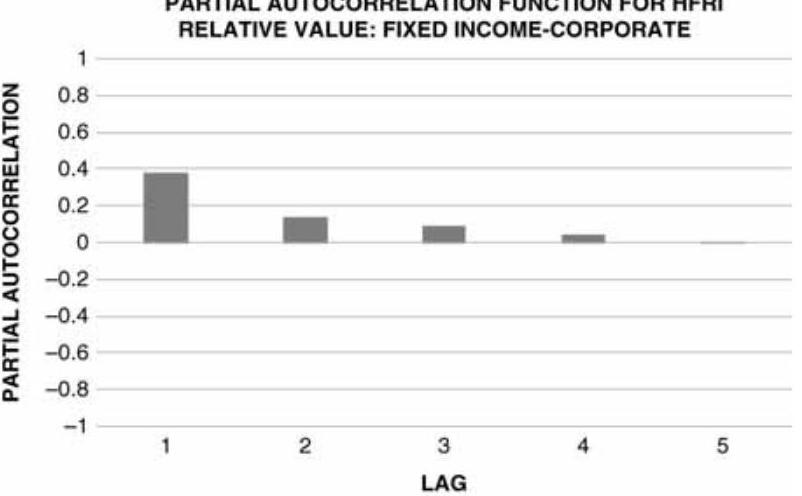
\includegraphics[max width=\textwidth]{2024_04_09_56e5743515a08e209ea4g-6}
\end{center}

Histogram of HFRI Relative Value: Fixed Income-Corporate Returns (Monthly) Jan. 2000-Dec. 2021

\begin{center}
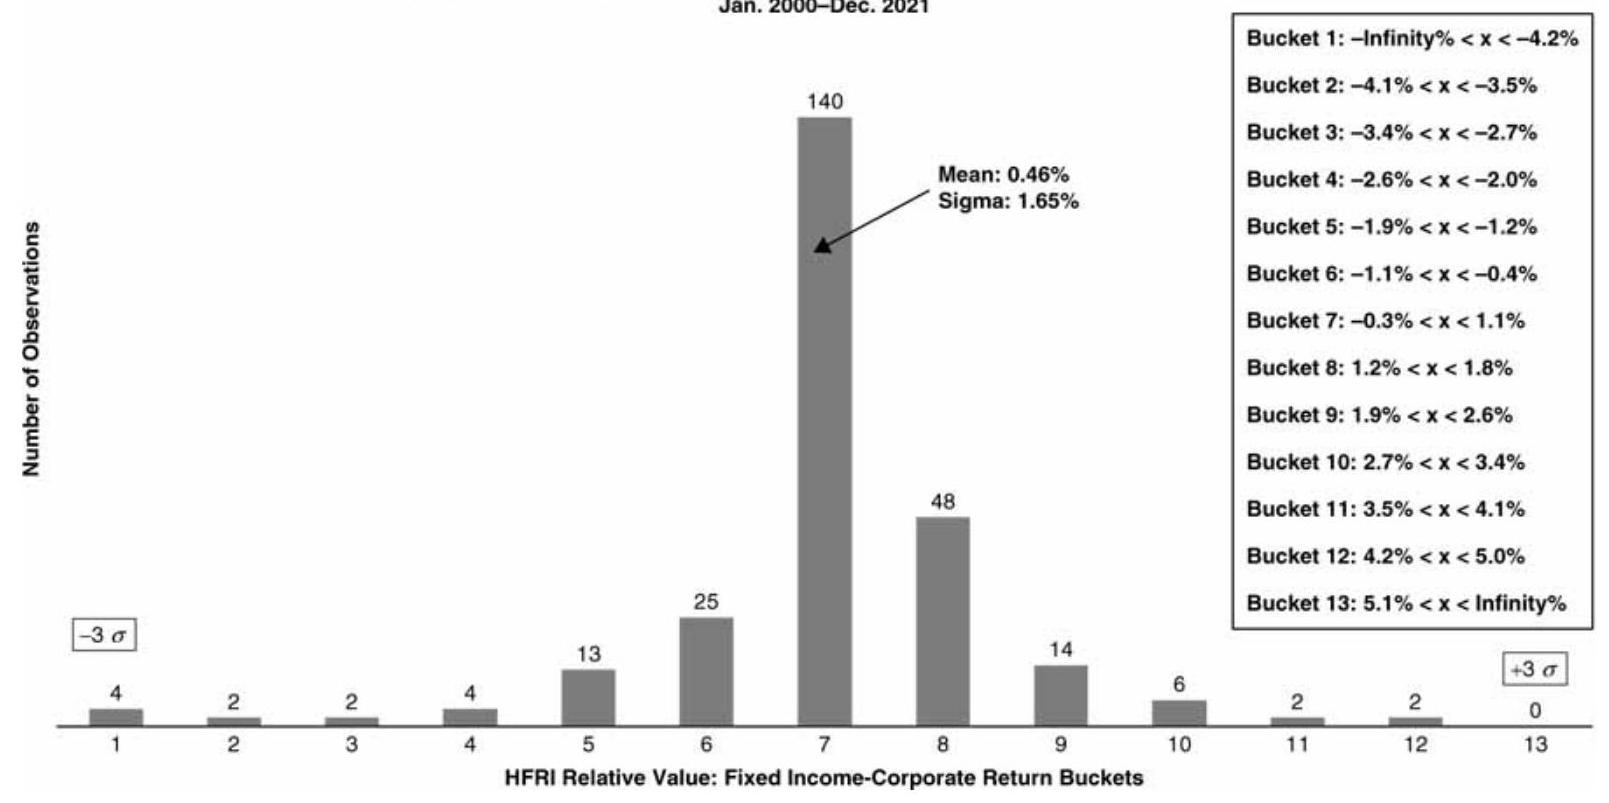
\includegraphics[max width=\textwidth]{2024_04_09_56e5743515a08e209ea4g-6(1)}
\end{center}

\section*{Statistical Summary of Returns}
Key observations on fixed-income arbitrage strategy returns that are consistent with economic reasoning are an essential component of knowledge and include the following:

\begin{enumerate}
  \item The historical return distribution of HFRI Fixed Income: Corporate exhibited moderately greater left skew and very high excess kurtosis relative to global equities.

  \item Volatility of returns was substantially lower than that of world equities.

  \item Returns exhibited strong positive first-order autocorrelation.

  \item Maximum drawdown was moderately milder than observed for global equities.

\end{enumerate}

\end{document}